\chapter{Cryptographic techniques for cybersecurity}


\section{Cryptography}

\begin{figure}[h]
    \centering
    \includegraphics[page = 2,trim = 0.5cm 3cm 1cm 5cm, clip, width = 0.55\textwidth]{\slides}
\end{figure}


The most used technique to achieve protection for many centuries is \textbf{cryptography}; a mathematical technique that involves algorithms for encryption and decryption:
\begin{itemize}
    \item the encryption algorithm takes a message (in clear) and transforms it in such a way that it becomes unintelligible;
    \item to recover the original text, the decryption algorithms make it readable again.
\end{itemize}
Next to the algorithms, \textbf{key-1} is needed for encryption and \textbf{key-2} for decryption, both of which are streams of bits.
Cryptography is used in communication and for data storage (for example, to store data on disks without permission to read them except for authorized users). The common terminology used in cryptography includes two other keywords:
\begin{itemize}
    \item \textbf{Plaintext} or \textbf{cleartext}: the unencrypted message, typically referred to as \textbf{P};
    \item \textbf{Ciphertext}: the encrypted message, typically referred to as \textbf{C}. Note that in some countries, the term "encrypted" may sound offensive for religious reasons (related to the cult of the dead); in such cases, "\emph{enciphered}" is preferred.
\end{itemize}


\subsection*{Cryptography's strength (Kerchoffs' principle)}
Kerckhoffs' Principle (1883) states that \ul{the security of a cryptosystem must lie in the choice of its keys only};
everything else (including the algorithm itself) should be considered of public knowledge.
However, this principle relies on the fact that the keys have the following properties.
\begin{itemize}
    \item Are kept \textbf{secret};
    \item Are managed only by \textbf{trusted systems};
    \item Are of \textbf{adequate length} % TODO: cross-reference this
\end{itemize}

If these properties are met,
not only it has no importance that the encryption and decryption algorithms are kept secret, but it is better to
make the algorithms public so that they can be widely analysed, and their possible flaws and vulnerabilities identified.

\subsection*{Security through obscurity (STO)}
The Kerckhoffs' Principle is related to the concept of \textbf{Security through obscurity}: it means that a system is protected, but the details on how it has been protected are not disclosed.\\
Generally, \ul{this alone is not considered a valid security mechanism} because if someone discovers how the system has been protected (and we have seen that there are also non-technical ways by which this can be achieved), it is no longer secure.

For this reason, we say that \emph{"Security through obscurity is as bad with computer systems as it is with women"}.
\begin{quote}
    "Men try to hide things from women, but when they discover the truth, it is worse than if they had known it from the beginning"
\end{quote}
\begin{flushright}
    (Antonio Lioy)
\end{flushright}
\emph{Editor's note:} don't hide things from your partner, regardless of gender.


However, there is a category of people (such as military men) which tend to apply STO, but as an \ul{additional
    layer}. It is possible to use STO as a layer only if a really strong algorithm is used (but not a secret one).



\section{Symmetric cryptography}
Depending on which relation exists between key-1 and key-2 there are different kinds of cryptography.

\subsection*{Secret key / symmetric cryptography}
\begin{figure}[h]
    \centering
    \includegraphics[page = 6,trim = 2.5cm 3cm 2.5cm 13cm, clip, width = 0.55\textwidth]{\slides}
    \caption{Symmetric cryptography}
    \label{fig:cap2slide6}
\end{figure}

It is so named because \textbf{only a single key} is shared by the sender and receiver. In the diagram, there is a plaintext used as input for the encryption (E) block, along with the key. The result is a comprehensible text that is transmitted to the receiver. To retrieve the original text, the decryption (D) block algorithm is used with the same key that was used for encrypting the initial text. If a different key is used, an output is generated, but it will be incorrect (and typically understandable).

The formulas used are as follows.

% TODO: fix these formulas 
\begin{align*}
    K_1 & = K_2 = K                                    \\
    C   & = enc(K,P) \quad \text{or} \quad C = \{P\} K \\
    P   & = dec(K,C) = enc^{-1} (K,C)
\end{align*}
Note that $C = \{P\} K$ means "encrypt the plaintext P using the key K".


% TODO: cross reference "Key distribution for symmetric cryptography"
The issue in the diagram (Figure \ref{fig:cap2slide6}) is represented by the dashed line: how can the key be securely shared between the sender and receiver?
We'll see it in \textit{Key distribution for symmetric cryptography}.


\subsection{Block algorithms}
\begin{figure}[h]
    \centering
    \includegraphics[page = 7,trim = 1cm 1.5cm 1cm 4cm, clip, width = 0.55\textwidth]{\slides}
    \caption*{Some famous symmetric encryption algorithms (block)}
\end{figure}

There are many algorithms, and the table on the left represents just a small selection. \\
The first column provides the name, the second indicates the key length, and the third specifies the basic unit each algorithm can encrypt. These algorithms are referred to as "\textbf{block algorithms}" because they operate on a fixed number of bits.

The \textbf{DES} algorithm, once a standard for many years, is now considered obsolete and should never be used.

The most commonly used algorithm of this kind is \textbf{AES}, currently recognized as the state of the art (the strongest).

\textbf{RC5} performs optimally when the block size is double the word size of the CPU architecture (e.g., 64-bit architecture -> 128-bit block) on which the algorithm is implemented.

Why are there so many algorithms? Because there are various types of computers, and many algorithms are not suitable for low CPU power.


\paragraph*{The EX-OR (XOR) function}
\begin{wrapfigure}{r}{0.255\textwidth}
    \centering
    \includegraphics[page = 8,trim = 21cm 7.2cm 0.5cm 8.5cm, clip, width = 0.25\textwidth]{\slides}
    \caption*{XOR function}
\end{wrapfigure}

It is the ideal "confusion" operator, available on all CPU. \\
The peculiarity of this truth table is that it has 50\% of
0 and 50\% of 1:
if XOR is performed with 2 random inputs (probability 0:1 = 50\% : 50\%),
then the output will also be equally random; while, for example, AND is more likely to produce 0.
That means that XOR does not change the probability distribution of the input, even though it generates different outputs.
Some properties:
\begin{itemize}
    \item if $A \oplus B = Z$ \\
          then $Z \oplus B = A$  or $Z \oplus A = B$
    \item $A \oplus 0 = A$ \\
          $A \oplus 1 = \overline{A}$\\
          $A \oplus A = 0$\\
          $A \oplus \overline{A} = 1$
\end{itemize}


\subsubsection{DES}
\textbf{DES} stands for "\textbf{Data Encryption Standard}" and it is a standard defined by \textit{FIPS 46/2} (Federal Information Processing Standard, the body responsible for setting standards for the American government). The modes for applying DES to data that is not equally divided into blocks are mentioned in the FIPS 81 standard.

DES is a unique algorithm because it has a 64-bit key, but its effective strength is equivalent to that of a \textbf{56-bit key}, as 8 bits are used for parity. This means that when a key is generated for the DES algorithm, only 56 bits are truly random, and every 7 bits, the algorithm inserts a bit that serves as the parity of the preceding 7 bits. When an attacker attempts to crack DES, they only need to discover these 56 truly random bits. DES is the only algorithm that distinguishes between actual (bits used to create the key) and effective (total number of bits) bits.

Developed in the 1960s, DES uses a \textbf{64-bit data block}, a size chosen when computers were less powerful. To perform all the necessary mathematical computations, a special-purpose unit called an \textbf{encryption processor} was created because DES relies on it to perform:

\begin{itemize}
    \item \textbf{XOR}: which is not a problem → elementary operation;
    \item \textbf{Shift}: not a problem → elementary operation;
    \item \textbf{Permutation}: expensive operation. The permutation is not random, there are several ones, but still implementing that was much more efficient if done directly in hardware.
\end{itemize}

\subsubsection{Triple DES (3DES, TDES)}
Triple DES is the repeated application of DES (three times). It is possible to use two or three different 56bit keys.
Typically, the process involves taking the input, encrypting it, and then repeating this operation two more times, using the output of the previous encryption as the input for the next encryption (resulting in three consecutive encryptions).

Normally, it is implemented in \textbf{EDE} mode, which, in its standard form, requires \ul{two keys}: the plaintext is first encrypted with key-1, then the decryption algorithm is applied to the output using key-2 (which does not actually decrypt but applies another transformation), and finally, this last output is encrypted again using key-1.
This mode was chosen because setting $K_1 = K_2 = K_3$ allows for the implementation of the simple DES in EDE mode.
Thus, both EEE and EDE work equally well. It has been shown that 3DES with two keys can have lower security guarantees than expected.

In particular, denoting $K_{eq}$ as the equivalent key obtained by applying the discussed transformations:
\begin{itemize}
    \item \textbf{3DES with 2 keys},
          \(K_{\text{eq}} = 56\) bits if $2^{59}B$ of memory is available, otherwise \(K_{\text{eq}} = 112\) bits:
          \[C' = \text{enc}(K_1, P) \quad C'' = \text{dec}(K_2, C') \quad C = \text{enc}(K_1, C'')\]
    \item \textbf{3DES with 3 keys}, \(K_{\text{eq}} = 112\) bits:
          \[C' = \text{enc}(K_1, P) \quad C'' = \text{dec}(K_2, C') \quad C = \text{enc}(K_3, C'')\]
\end{itemize}

The 3DES is a standard FIPS 46/3 and ANSI X9.52 (family X9 is standard for security in banking and financial
applications).

\begin{figure}[h]
    \centering
    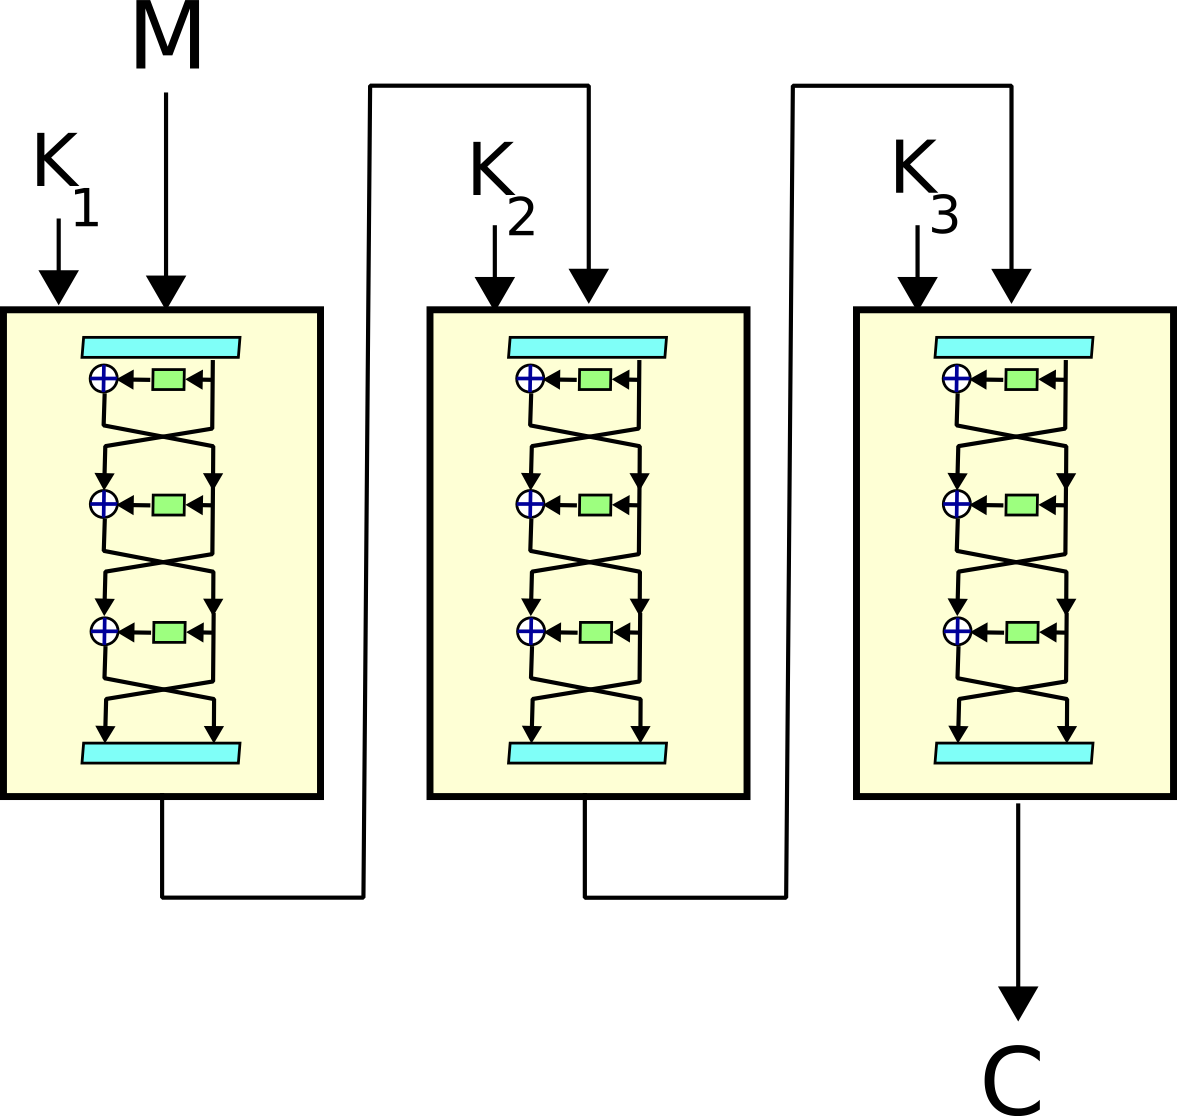
\includegraphics[width = 0.30\textwidth]{chapter2/3des.png}
\end{figure}

\paragraph*{Why not Double DES?}
The double application of any encryption algorithm is susceptible to a \textbf{known-plaintext} attack known as \textit{meet-in-the-middle} see below), which allows for the decryption of data with at most \(2^{N+1}\) attempts (if the keys are \(N\) bits long), instead of the $2^{2n}$ steps one would expect from an ideally secure algorithm with $2n$ bits of key.
If the attacker knows one plaintext, they can execute the attack. For this reason, \textbf{the double version of encryption algorithms is never used} because the computation time doubles, but the effective key length increases by just one bit.

Furthermore, it has been proven that if the base symmetric algorithm is a \href{https://en.wikipedia.org/wiki/Group_(mathematics)}{\underline{group}} , then there exists an equivalent key \(K_3\) such that:

\[
    \text{enc}(K_2, \text{enc}(K_1, P)) = \text{enc}(K_3, P)
\]

This implies that in this case, the time needed for normal encryption/decryption doubles, but not a single bit is gained in terms of \(K_{eq}\).


\subparagraph*{Meet-in-the-middle attack}\label{meetinthemiddle}
By hypothesis, N-bit keys are used, and we have known plaintext (\(P\)) and ciphertext (\(C\)) such that 
\[C = \text{enc}(K_2, \text{enc}(K_1, P))\]. \\
Note that \(\exists M\) such that  
\[
    M = \text{enc}(K_1, P)\\
    C = \text{enc}(K_2, M)
\]
\\
The attacker computes \(2^N\) values \(X_i = \text{enc}(K_i, P)\) and then computes \(2^N\) values \(Y_j = \text{dec}(K_j, C)\).
The search then involves finding those values \(K_i\) and \(K_j\) such that \(X_i = Y_j\).
There can be "false positives" but these can be easily discarded if more than one \((P, C)\) pair is available.

Let's consider a company protecting its communication between Turin and Milan using double DES. If the attacker sniffs the network (and reads the encrypted data), they can send a message over that line (meaning they control the plaintext), and then observe the ciphertext (of the sent plaintext) automatically generated by the security system.
This is a way to obtain a pair of \((P, C)\) without knowing the keys.

\begin{figure}[h]
    \centering
    \includegraphics[page = 12,trim = 3cm 3cm 2cm 3cm, clip, width = 0.50\textwidth]{\slides}
\end{figure}


\newpage
\subsection{Application of block algorithm}

\textit{How is a block algorithm applied to a data quantity different from the algorithm's block size?}
There are two cases:
\begin{enumerate}
    \item Data size to encrypt $>$ algorithm's block size
          \begin{itemize}
              \item \textbf{ECB (Electronic Code Book):} Nowadays considered not secure and must never be used.
              \item \textbf{CBC (Cipher Block Chaining):} Currently the best way to apply an encryption algorithm to data that is bigger than the size of the algorithm's block size.
          \end{itemize}

    \item Data size to encrypt $<$ algorithm's block size
          \begin{itemize}
              \item \textbf{Padding:} Used only when the data size is not exactly a multiple of one block size (e.g., when data is 2.6 blocks long). Note that this technique is not used to pad data that is just shorter than one block size. 
              \begin{itemize}
                \item \textbf{CTS (CipherText Stealing):} Permits the use of block algorithms without padding, avoiding an increase in the size of the ciphertext compared to the plaintext.
              \end{itemize}
              \item \textbf{CFB (Cipher FeedBack), OFB (Output Feedback), CTR (Counter mode):} These are application modes for an algorithm, not algorithms themselves.
          \end{itemize}
\end{enumerate}
\textbf{ATTENTION!} These are NOT algorithms; they are application modes for an algorithm.

It is necessary to specify: 
the algorithm, the size of key, and if it is a block algorithm, also the mode of the application (e.g., AES-128-CBC).


\subsubsection{ECB}
\paragraph*{Encryption}
This mode splits the plaintext into blocks, and each block is encrypted separately with the key; 
that means that, for each block \(i = 0, \ldots, N\),
\[
C_i = \text{enc}(K, P_i) 
\]
\begin{figure}[h]
    \centering
    \includegraphics[page = 14,trim = 8cm 2cm 8cm 12cm, clip, width = 0.30\textwidth]{\slides}
    \caption*{Encryption with ECB}
\end{figure}

\underline{It must \textbf{NOT} be used!} [\textit{Lioy said that the exam will not be passed if ECB is used somehow}]. 
In particular, it must not be used on long messages (any message longer than 1 block) because:
\begin{itemize}
  \item If the attacker is intercepting the ciphertext and exchanges the position of 2 blocks, it is not detected (\textbf{block swapping}). This permits to exchange data inside an encrypted message;
  \item Identical blocks generate identical ciphertexts, hence it is vulnerable to \textbf{known-plaintext attacks}. Plaintext attacks require the precomputation of all possible encryptions of a known plaintext: comparing the encrypted block with all the precomputed possible encryptions, it is possible to figure out what the key is.  
\end{itemize}

\subparagraph*{Known-plaintext attack example}
Let us suppose that we want to intercept a message sent by the rector of the Politecnico di Torino. It is possible
to assume that his messages will contain the word “Torino”, so we start encrypting this word with all possible
keys. Next, we can go sniffing the blocks sent by the rector: if any of these blocks is equal to the encryption
of “Torino”, then we can use the key used to obtain that encryption of “Torino” to decrypt the rest of the
message. Some arguments against this method could be: in which way is “Torino” written (e.g., “TORINO”,
“Torino”)? What if “Torino”, since it is shorter than one machine word, is split into different blocks (e.g., \(P_i\) =
“…To”, \(P_{i+1}\) = “rino…”)? The known-plaintext attack is made possible by the fact that usually people exchange
data in a structured format, so that there are metadata that are usually known (e.g., fixed header).


If a Word file is created with just a word, it is big KBs of memory (and not just bytes). This happens because
Word applies a header on the document which is always the same (and always at the beginning of a file). If
the first block of a Word file is encrypted, it can serve as a dictionary for Word files. This means that we do not
even have to guess some plaintext, but just the file format.


\paragraph*{Decryption}
Decryption is a straightforward process as it involves taking the ciphertext block and decrypting it with the corresponding key. In the case of an error in transmission, it only affects the decryption of that specific block, and \textbf{there is no propagation of the error to other blocks}.
For each block \(i = 0, \ldots, N\), 
\begin{itemize}
    \item $P_i = \text{enc}^{-1}(K, C_i)$
\end{itemize}
\begin{figure}[h]
    \centering
    \includegraphics[page = 15,trim = 8cm 2cm 8cm 10.5cm, clip, width = 0.30\textwidth]{\slides}
    \caption*{Decryption with ECB}
\end{figure}


\subsubsection{CBC (Cipher Block Chaining)}

\paragraph*{Encryption}
This mode resolves all of ECB's problems.
It divides the plaintext into blocks, but before each block is encrypted, it is \textbf{XORed with the ciphertext of the previous block}. 
This introduces unpredictability in the encryption process.
However, there is an issue with the first block (which serves as the header of the mentioned file); to apply CBC, an additional element called the \textbf{Initialization Vector (IV)} must be introduced, considered as \(C_0\), with the sole purpose of altering the first plaintext block. 

CBC also provides protection against block swapping because if blocks are swapped, the output will be different due to being altered with the incorrect XOR element.
\[
C_i = \text{enc}(K, P_i \oplus C_{i-1})
\]

\begin{figure}[H]
    \centering
    \includegraphics[page = 16,trim = 4cm 2cm 4cm 8.5cm, clip, width = 0.55\textwidth]{\slides}
    \caption*{CBC decryption}
\end{figure}


\paragraph*{Decryption}
The IV vector needs to be known at the receiver as well because, when the ciphertext is received, the IV must be known to decrypt the first block (since XOR is the inverse operator of itself). 
The IV must also be different every time (hopefully random) to avoid being guessed, as its purpose is to make it impossible to precompute the possible encryptions of the first block. 
It must also be a \textbf{NONCE} (Number used once), meaning that the IV should be generated and never reused in the future.

In some cases, the IV is sent in clear because even if the attacker knows it, they could start the computation only at that moment, and this is a time-consuming task. Moreover, it will permit the attacker to attack only the sent message, as the next one will have another IV. 
The IV can also be sent encrypted using ECB since it is just a block.

\[
    P_i = \text{enc}^{-1}(K, C_i ) \oplus C_{i-1}
\]

\begin{figure}[H]
    \centering
    \includegraphics[page = 16,trim = 4cm 2cm 4cm 8.5cm, clip, width = 0.55\textwidth]{\slides}
    \caption*{CBC decryption}
\end{figure}



\subsubsection*{Padding (aligning, filling)}
\begin{figure}[H]
    \centering
    \includegraphics[page = 18,trim = 3.5cm 7cm 3.5cm 9cm, clip, width = 0.55\textwidth]{\slides}
\end{figure}
It is not always possible to have the plaintext split into blocks that are all the same size. In the picture, the data consists of two complete blocks and a partial block at the end. To encrypt this small part, a technique called padding is used. Bits are added at the end of the original data until it reaches a multiple of a block.
However, it has some problems since:
\begin{itemize}
    \item The ciphertext gets longer than the plaintext: adding useless data means transmitting / storing more data
    than needed;
    \item Which should be the value of padding bits? How can we distinguish the padding from the original
    plaintext at the receiver?
\end{itemize}

\paragraph*{Padding Techniques:}
\begin{itemize}
    \item If the length is known or it can be obtained as in the case of a C string, it is possible to add null bytes
    at the end: \texttt{0x00 0x00 0x00};
    \item The original DES specified to add one "1" bit followed by as many "0" as needed: \texttt{1000000};
    \item One byte with value 128 followed by null bytes: \texttt{0x80 0x00 0x00};
    \item Last byte's value equal to the length of padding: \texttt{0x?? 0x?? 0x0} (3 bytes of padding. The last one
    has value 3, and the previous has a value to be specified).
\end{itemize}

There are numerous padding techniques available, and the choice of a specific padding method plays a crucial role in preventing or mitigating various types of attacks. 

There are many kinds of values that can be selected (\textit{do not remember all the techniques, just remember there
are many and the proper one must be selected}):

\begin{itemize}
    \item (Schneier) null bytes, e.g., \texttt{0x00 0x00 0x03}
    \item (SSL/TLS) bytes with value $L$, e.g., \texttt{0x03 0x03 0x03}
    \item (SSH2) random bytes, e.g., \texttt{0x05 0xF2 0x03}
    \item (IPsec/ESP) progressive number, e.g., \texttt{0x01 0x02 0x03}
    \item Byte with value $L-1$, e.g., \texttt{0x02 0x02 0x02}
\end{itemize}


\paragraph*{Some notes}
\begin{itemize}
    \item $B$ stands for the size of the algorithm's block
    \item $D$ stands for the size of data to process
\end{itemize}

Some of these techniques offer (minimal) integrity control: if the key is wrong or data is manipulated, then the
padding bytes are incoherent (e.g., length of something bigger than one block or wrong padding values).\\
Typically, this is applied to large data, on the last fragment resulting from the division into blocks (e.g., for ECB
or CBC). If $|D| < |B|$, an ad-hoc technique is preferred (CFB, OFB, CTR, …). If there is just a byte, it is not
good to add 65 bytes of padding.\\
Even if the plaintext is an exact multiple of the block, padding must be added anyhow to avoid errors in the
interpretation of the last block. The biggest padding is required when there is no padding to add.\\
With SSH2, padding equal to data gives different ciphertexts (even when encrypted with the same key).\\
The padding type for a certain algorithm determines the type of (some) possible attacks, but it also depends
upon the algorithm used.

\subsubsection{Ciphertext stealing (CTS)}
When using padding, the size of the ciphertext is bigger than the plaintext. This may not be acceptable in
several cases (for example, data encrypted on a hard disk that may not fit on the same disk). It is possible to use
CTS instead of padding. The last (partial) block is filled with bytes taken from the second-to-last block
(encrypted), then these bytes are removed from the second-to-last block (which becomes a partial one). After
encryption, the positions of the last and second-to-last blocks are exchanged.

It is useful when it is not possible to increase the size of data after encryption, but the computation time slightly increases.


\paragraph*{CTS Example with ECB (encryption)}
\begin{figure}[h]
    \centering
    \includegraphics[page = 23,trim = 2cm 1.5cm 0.4cm 4cm, clip, width = 0.55\textwidth]{\slides}
\end{figure}
\begin{enumerate}
    \item The plaintext is split into blocks;
    \item The second-to-last block is full, so it is possible to encrypt it with the key;
    \item The last one is not full and creates a problem;
    \item The encrypted block $C_{n-1}$ is split into two parts: \textit{head} and \textit{tail}. The tail has the same size as the part that is missing in the last block;
    \item The tail is added to the partial block, creating a full block;
    \item The fully created block is transmitted, and then the head is transmitted.
\end{enumerate}
The receiver must reverse the procedure. Bits corresponding to the tail are encrypted twice.\\ \ul{Exchanging the blocks is necessary because if we send the head without the tail, then the beginning of the next block is interpreted as part of the previous one.}


\paragraph*{CTS Example with CBC (encryption)}
\begin{figure}[h]
    \centering
    \includegraphics[page = 23,trim = 2cm 1.5cm 0.4cm 4cm, clip, width = 0.55\textwidth]{\slides}
\end{figure}
